% ===========================================================================
%  本科毕业论文 LaTeX 模板
%  编译方式：pdflatex -> bibtex -> pdflatex -> pdflatex
%  或直接使用 latexmk -pdf main.tex
%
%  目录结构：
%    main.tex            主控文件（页面、字体、标题、页码、目录样式）
%    chapters/           正文章节
%      introduction.tex      第 1 章  绪论
%      related_work.tex      第 2 章  相关理论与技术基础
%      method.tex            第 3 章  方法设计
%      experiment.tex        第 4 章  实验与结果分析
%      conclusion.tex        第 5 章  总结与展望
%    images/             插图（png/eps/jpg 均可）
%    references.bib      参考文献数据库
%    cover.pdf           封面（学校统一格式，2 页）
%
%  使用前请确认：已在 cover.pdf 中替换为自己的姓名、学号、专业与题目。
% ===========================================================================

\documentclass[12pt,a4paper,UTF8]{ctexart}

\usepackage{graphicx}
\usepackage{amsmath}
\usepackage{amsfonts}
\usepackage{amssymb}
\usepackage{xcolor}
\newcommand{\upcite}[1]{\textsuperscript{\cite{#1}}}

\usepackage[
colorlinks=true,
linkcolor=black,
citecolor=black,
bookmarks=false
]{hyperref}

\usepackage{booktabs}
\usepackage{pdfpages}
\usepackage[nottoc]{tocbibind}
\usepackage{tocloft}

% ===== 各级目录添加虚线 =====
\renewcommand{\cftsecleader}{\cftdotfill{\cftdotsep}}
\renewcommand{\cftsubsecleader}{\cftdotfill{\cftdotsep}}
\renewcommand{\cftsubsubsecleader}{\cftdotfill{\cftdotsep}}

% ===== 目录整体居中配置 =====
\renewcommand{\cfttoctitlefont}{\hfil\bfseries\fontsize{15}{18}\selectfont}
\renewcommand{\cftaftertoctitle}{\hfil}
\newlength{\tocwidth}
\setlength{\tocwidth}{20cm} % 目录内容总宽度，按需微调

\usepackage{multirow}
\usepackage{geometry}
\usepackage[table]{xcolor}
\usepackage{enumitem}
\usepackage{tikz}
\usetikzlibrary{positioning,arrows.meta}

\hbadness=10000
\hfuzz=5pt

\geometry{
a4paper,
top=3.3cm,
bottom=2.3cm,
left=2.8cm,
right=2.3cm
}

\usepackage{chngcntr}

\usepackage{setspace}
\linespread{1.5}

\usepackage{caption}
\captionsetup[figure]{labelsep=space}
\captionsetup[table]{labelsep=space}

\usepackage{indentfirst}
\setlength{\parindent}{2em}

\usepackage{newtxtext,newtxmath}

\CJKfamily{song}
\fontsize{12}{18}\selectfont

\usepackage{titlesec}

\titleformat{\section}
{\centering\bfseries\fontsize{15}{18}\selectfont}
{\thesection}{1em}{}

\titleformat{\subsection}
{\bfseries\fontsize{14}{16.8}\selectfont}
{\thesubsection}{1em}{}

\titleformat{\subsubsection}
{\bfseries\fontsize{12}{14.4}\selectfont}
{\thesubsubsection}{1em}{}

\setcounter{secnumdepth}{3}
\setcounter{tocdepth}{3}

\usepackage{fancyhdr}

\pagestyle{fancy}
\fancyhf{}
\renewcommand{\headrulewidth}{0pt}
\renewcommand{\footrulewidth}{0pt}
\cfoot{\fontsize{9}{10.8}\selectfont \thepage}
\setlength{\footskip}{10mm}

% 重定义目录：标题居中+内容块居中
\makeatletter
\renewcommand{\tableofcontents}{%
\section*{\contentsname}
\@mkboth{\MakeUppercase\contentsname}{\MakeUppercase\contentsname}
\centering
\begin{minipage}{\tocwidth}
    \@starttoc{toc}
\end{minipage}
}
\makeatother

\title{【论文中文题目】}
\author{【作者姓名】}
\date{\today}
\begin{document}

% ----------------【封面：两页彻底无页码】----------------
\cleardoublepage
\pagestyle{empty}

\includepdf[
pages=1-2,
pagecommand={\pagestyle{empty}},
fitpaper
]{cover.pdf}
\cleardoublepage
\pagestyle{fancy}

% ---------------- 任务书（学校统一格式，按需插入）----------------
% 如需插入任务书，取消下行注释，并把 task.pdf 放到本目录下：
% \clearpage
% \pagestyle{empty}
% \pagenumbering{gobble}
% \includepdf[pages=1-3]{task.pdf}

% ---------------- 中文摘要 i：标题在上，摘要二字在标题下面 ----------------
\newpage
\pagestyle{fancy}
\pagenumbering{roman}
\setcounter{page}{1}

\begin{center}
\bfseries
\fontsize{16}{19.2}\selectfont
【论文中文题目】
\end{center}

\vspace{0.1em}
\section*{摘\quad 要}
\addcontentsline{toc}{section}{摘\quad 要}

\vspace{0.5em}
【中文摘要】此处填写论文中文摘要，建议篇幅 300$\sim$500 字。摘要应能独立成篇，一般依次包含以下四部分内容：（1）研究背景与意义；（2）采用的方法与技术路线；（3）完成的主要工作与创新点；（4）实验结果与结论。摘要中不宜出现图表、公式与参考文献标注。

\vspace{1em}
{\bfseries 关键词：}
关键词一；关键词二；关键词三；关键词四；关键词五

% ---------------- 英文摘要 ii：英文题目在上，Abstract在题目下方 ----------------
\newpage

\begin{center}
\bfseries
\fontsize{16}{19.2}\selectfont
[Title of Thesis in English]
\end{center}

\vspace{1em}
\section*{Abstract}
\addcontentsline{toc}{section}{Abstract}

\vspace{0.5em}
[Abstract] Write the English abstract here; 300--500 words is recommended. It should be self-contained and cover: (1) research background and significance; (2) the proposed method and technical route; (3) main contributions; (4) experimental results and conclusions. Figures, tables, equations and citation marks should not appear in the abstract.

\vspace{1em}
{\bfseries Key words:}
Keyword 1; Keyword 2; Keyword 3; Keyword 4; Keyword 5

% ---------------- 目录无页码 ----------------
\newpage
\pagenumbering{gobble}
\pagestyle{empty}
\tableofcontents

% ---------------- 正文从阿拉伯1开始 ----------------
\newpage
\pagestyle{fancy}
\pagenumbering{arabic}
\setcounter{page}{1}

\section{绪论}

\subsection{研究背景与意义}

【阐述研究背景与选题意义，建议 2～3 段。】

随着……技术的快速发展，……在……领域得到了广泛应用\upcite{lecun2015deep}。然而，现有方法仍存在以下不足：其一，……；其二，……；其三，……。因此，针对上述问题开展研究，具有重要的理论意义与实际应用价值。

\subsection{国内外研究现状}

【梳理国内外相关工作，简述代表性方法，并在末尾指出其不足。】

针对该问题，文献\upcite{vaswani2017attention}提出了……方法，通过……实现了……；文献\upcite{devlin2019bert}进一步……。国内学者在……等方面也开展了大量研究\upcite{zhongwen2020shili}。综合来看，现有研究在……方面仍存在改进空间，这正是本文工作的切入点。

\subsection{本文主要工作}

本文围绕【研究主题】展开研究，主要工作包括以下三个方面：

\begin{enumerate}
  \item 针对【问题一】，提出了【方法或模型名称】，通过【关键技术】解决【具体困难】；
  \item 针对【问题二】，设计了【模块或策略名称】，实现了【预期效果】；
  \item 在【数据集或实验平台】上完成了对比实验与消融实验，验证了所提方法的有效性。
\end{enumerate}

\subsection{论文组织结构}

全文共分为五章：第 1 章绪论，介绍研究背景与意义，梳理国内外研究现状，并给出本文的主要工作与组织结构；第 2 章相关理论与技术基础，介绍本文涉及的基础理论与关键技术；第 3 章方法设计，给出总体设计方案与各关键模块的具体设计；第 4 章实验与结果分析，介绍实验设置，并通过对比实验与消融实验验证所提方法的有效性；第 5 章总结与展望，总结全文工作并指出未来研究方向。


\clearpage
\section{相关理论与技术基础}

本章介绍与本文研究密切相关的基础理论与关键技术，为后续章节的方法设计提供理论支撑。

\subsection{基础理论}

【介绍本文所依赖的一至两个基础理论，说明其基本原理及其在本研究中的作用。】

以……为例，其核心思想可以形式化描述为：
\begin{equation}
  y = f(x;\theta)
\end{equation}
其中 \(x\) 为输入，\(\theta\) 为待学习参数，\(f(\cdot)\) 表示……。

\subsection{关键技术}

【介绍本文用到的一至两项关键技术，说明其原理、优势与适用场景。】

……\upcite{he2016resnet}。该技术的优势在于……，但也存在……的局限。本文在此基础上进行了改进，具体方案见第 3 章。

\subsection{本章小结}

本章对……等基础理论与关键技术进行了介绍，为第 3 章的方法设计奠定了理论基础。


\clearpage
\section{方法设计}

本章给出本文方法的总体设计方案，并对各关键模块进行详细说明。

\subsection{总体设计方案}

【先用一段文字概括整体思路与技术路线，再给出总体框架图并对照图说明各部分的衔接关系。】

本文方法的总体框架如图 \ref{fig:overall} 所示，整体流程包括【阶段一】、【阶段二】与【阶段三】三个部分。首先，……；其次，……；最后，……。

\begin{figure}[htbp]
    \centering
    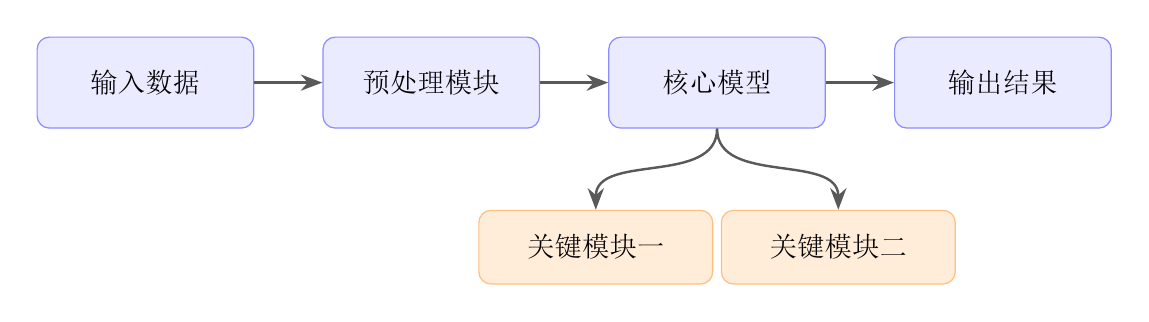
\includegraphics[width=0.9\textwidth]{images/overall_framework.png}
    \caption{总体框架图（示例，请替换为本人论文的框架图）}
    \label{fig:overall}
\end{figure}

\subsection{关键模块设计}

【分模块介绍设计细节，每个模块单独成段，必要时配合公式、伪代码或示意图说明。】

以【关键模块一】为例，其计算过程可以表示为：
\begin{equation}
  \mathbf{h} = \sigma\left(\mathbf{W}\mathbf{x} + \mathbf{b}\right)
\end{equation}
其中 \(\mathbf{W}\) 与 \(\mathbf{b}\) 为可学习参数，\(\sigma(\cdot)\) 为激活函数。

【关键模块二】的设计目标是……，具体实现上……。

\subsection{本章小结}

本章介绍了所提方法的总体设计与各关键模块的实现方式，下一章将通过实验对方法的有效性进行验证。


\clearpage
\section{实验与结果分析}

\subsection{实验环境与数据集}

【列出硬件环境、软件环境与所用数据集的基本信息。】

实验硬件环境为……，软件环境为……。实验采用……数据集，该数据集包含……条样本，按 …… 的比例划分为训练集、验证集与测试集。

\subsection{实验结果与分析}

【给出对比实验与消融实验的结果表，并对表中数据进行分析，说明各模块的贡献。】

为验证所提方法的有效性，本文选取……作为对比方法，评价指标采用……。实验结果如表 \ref{tab:result} 所示。

\begin{table}[htbp]
  \centering
  \caption{对比实验结果（示例，请替换为本人论文的实验结果）}
  \label{tab:result}
  \vspace{0.8em}
  \renewcommand{\arraystretch}{1.3}
  \begin{tabular}{lccc}
    \toprule
    \textbf{方法} & \textbf{指标一} & \textbf{指标二} & \textbf{指标三} \\
    \midrule
    基线方法 A & 0.0000 & 0.0000 & 0.0000 \\
    基线方法 B & 0.0000 & 0.0000 & 0.0000 \\
    本文方法   & \textbf{0.0000} & \textbf{0.0000} & \textbf{0.0000} \\
    \bottomrule
  \end{tabular}
\end{table}

由表 \ref{tab:result} 可见，……。为进一步验证各模块的作用，本文还进行了消融实验，结果显示……。

\subsection{本章小结}

本章介绍了实验设置，并通过对比实验与消融实验验证了所提方法的有效性。


\clearpage
\section{总结与展望}

\subsection{本文工作总结}

【概括本文完成的主要工作与取得的结果，与第 1 章提出的研究内容相呼应。】

本文针对……问题开展了研究，主要完成了以下工作：……。实验结果表明，……。

\subsection{未来工作展望}

【指出当前研究的局限，并展望后续可以继续深入的方向。】

本文工作仍存在一些不足：……。未来可以从以下几个方向继续完善：其一，……；其二，……；其三，……。


\clearpage

% ---------------- 参考文献 ----------------
\clearpage
\begin{fontsize}{10.5}{12.6}\selectfont
\sloppy
\bibliographystyle{unsrt}
\bibliography{references}
\fussy
\end{fontsize}

% ---------------- 致谢 ----------------
\clearpage
\section*{致\quad 谢}
\addcontentsline{toc}{section}{致\quad 谢}

【致谢正文】在此向指导教师、学院老师、同窗与家人表达感谢。一般依次感谢：指导教师在选题、研究思路与论文撰写过程中的具体指导；学院与实验室提供的条件支持；同学间的讨论与帮助；家人的理解与支持。落笔宜真诚具体，避免空泛套话。


% ---------------- 附件（无页码，载入完整 PDF 的所有页面）----------------
% 附件通常包括：外文文献翻译、文献复印件、程序清单、原始数据等。
% 请把附件 PDF 放到本目录下，并把文件名替换到下面的 \includepdf 中。
% 若暂时没有附件，保持以下两行注释即可，不影响编译。
%
% \clearpage
% \pagestyle{empty}
% \pagenumbering{gobble}
% \includepdf[pages=-]{appendix-translation.pdf}   % 外文翻译
% \includepdf[pages=-]{appendix-paper.pdf}         % 文献复印件


\end{document}